\documentclass{article}

\usepackage[margin=1in]{geometry} % full-width

% AMS Packages
\usepackage{amsmath}
\usepackage{amsthm}
\usepackage{amssymb}
\usepackage[caption=false,font=normalsize]{subfig}
\usepackage{array}
\usepackage{graphicx}
\usepackage{multirow, makecell}
\usepackage{booktabs} %%% for toprule, bottomrule in tables

% Unicode
\usepackage[utf8]{inputenc}
\usepackage[hyphens]{url}
\usepackage{hyperref}
\hypersetup{breaklinks=true}
\urlstyle{same}
\usepackage{matlab-prettifier}

\usepackage{cite}
\lstset{
  style              = Matlab-editor,
  basicstyle         = \mlttfamily,
  escapechar         = ",
  mlshowsectionrules = true,
}
% Natbib
\bibliographystyle{ieeetr}

\graphicspath{{Figures/}}

% Author info
\title{Effectiveness of Belleville Washers for Seismic Retrofit of Substation Equipment}
\author{Author One$^1$\thanks{Author One was partially supported by Grant XXX} \and Author Two$^2$ \and Author Three$^1$}

%\date{
%	$^1$Organization 1 \\ \texttt{\{auth1, auth3\}@org1.edu}\\%
%	$^2$Organization 2 \\ \texttt{auth3@inst2.edu}\\[2ex]%
%	\today
%}
\setlength{\parindent}{0pt}

\newcommand{\Mspool}{M_\text{spool}}
\newcommand{\xtddot}{\ddot{x}_\text{t}}
\newcommand{\thetaw}{\theta_\text{w}}
\newcommand{\MCVT}{M_\text{CVT}}
\newcommand{\hCG}{h_\text{CG}}
\newcommand{\Izero}{I_\text{0}}

\begin{document}
	\maketitle
	
\begin{abstract}
Seattle City Light (SCL), a power utility in the Pacific Northwest where there is potential for large earthquakes, has retrofitted several Capacitive Voltage Transformers (CVT) in their substations with Belleville washer arrangements at the bases to improve seismic performance. The strategy is simple and relatively low-cost to implement, and preliminary testing at SCL has demonstrated improved seismic performance. The washer arrangements essentially function as seismic isolators, reducing the frequency and increasing damping. To expand the implementation of this strategy more broadly for other equipment and at other utilities’ substations, this project systematically characterizes the stiffness and damping mechanisms of Belleville washer arrangements and tests a retrofitted 230kV CVT on an earthquake simulator. Special instrumentation is developed to monitor the mechanics of the Belleville washer arrangements including force, deformation and equipment base moment measurements. A detailed modeling and analysis procedure is developed, allowing for either a nonlinear dynamic approach or an equivalent linear dynamic approach, to predict the response of equipment such as CVTs outfitted with Belleville washer stacks for seismic protection. The analysis procedure has been validated with experimental measurements. Essentially, knowing the force-deformation response of a washer configuration, obtained for example by cyclic loading in a material testing machine, together with the inertia characteristics of the equipment, the seismic response of the equipment can be predicted. This will enable washer configurations to be designed and deployed readily for seismic protection of various equipment.
\vspace{\baselineskip}	

\noindent\textbf{Keywords:} Substation equipment, seismic performance improvement, nonlinear and linear dynamic analysis, Belleville washers (disc springs), damping, experimental validation
\end{abstract}

	
\section{Introduction}	\label{sec:intro}
\subsection{Background and objectives}
Base isolation and supplemental damping systems are now widely used as seismic protective systems in structures. They represent a design philosophy that seeks to reduce seismic demand on functional structural components, and to minimize if not eliminate damage and permanent deformation even under large earthquakes. This is in contrast to the conventional seismic design philosophy, wherein structural components are designed to be ductile, and undergo permanent deformation without failure. For critical structures and equipment, such as in electrical substations, the approach of reducing seismic demand and permanent deformations is more attractive to ensure continued functioning of such structures and equipment post-earthquake. The concept of frequency modification for substation equipment was recommended as early as 1973 in a report prepared for Bonneville Power Administration (BPA) \cite{couch1973procedures}. Base isolation and supplemental damping systems are being increasingly deployed in substations for seismic protection \cite{cochran2015seismic, Kempner2015isolation, oikonomou2016seismic, saadeghvaziri2009seismic}.\\

One approach to modifying frequency and adding damping is using stacks of Belleville washers. Belleville washers, named after Julian Belleville, who patented them in 1867, are circular washers given a taper to form a conical shape (Figure \ref{fig:Onewasher}). They are also known as a disc springs or conical spring washers, although the term “disc springs” may be more appropriate \cite{NBlunt} for the type of dynamic application considered in this report. When a compressive load is applied along the axis, the washer flattens by way of elastic deformation, resulting in spring action \cite{shigley2004standard}. 
When washers are nested such that the bottom surface of one is placed on the top surface of the next, frictional rubbing between these surfaces results in hysteretic behavior (see section \ref{sec:washerstackforcedisp}), and hence energy dissipation. The washers can also be stacked in different ways as illustrated in Figures \ref{fig:Washerstack} and \ref{fig:WasherNomenclature}. Thus the stiffness and dissipation of a stack of Belleville washers can be tuned. Testing discussed further in section \ref{sec:washerstackforcedisp} has shown that the force-displacement hysteresis of washer stacks is stable and repeatable. These stacks therefore lend themselves to modeling, and use as engineered frequency modification and energy dissipation devices. For early analyses of the mechanical behavior of Belleville washers, see \cite{ashworth1946disk, almen1936uniform}, considering both single washer and nesting. For a more recent study on the analysis of washer mechanical behavior, see \cite{zhou2023modeling} and the references therein. The force-displacement behavior of a single washer 
is given by \cite{shigley2004standard, almen1936uniform}

\begin{figure}
\centering
\hfil
\subfloat[Shape and dimension specifications (source: \cite{shigley2004standard})]{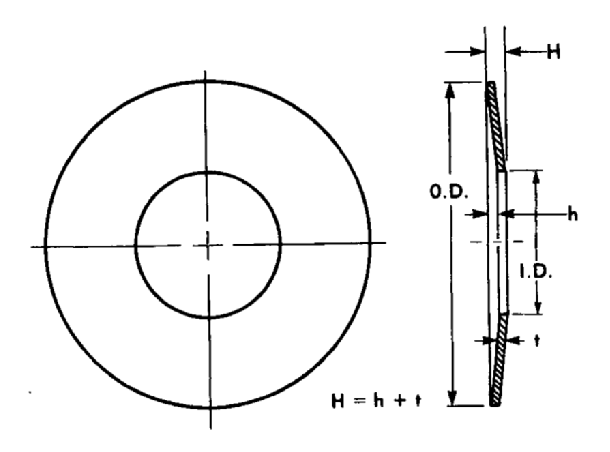
\includegraphics[scale=0.8]{Onewasher.eps}%
\label{fig:Onewasher}}
\hfil
\subfloat[Example of a stack with series-parallel arrangement]{\raisebox{1.2em}{\includegraphics[scale=1]{Photo_2units2U2D.eps}%
\label{fig:Photo2units2U2D}}}
\caption{Belleville washer shape, dimensions and stack consisting of series-parallel arrangement}
\label{fig:Washerstack}
\end{figure}


\begin{equation}\label{eqn:forcedispwasher}
  F=\frac{E\delta}{(1-\mu^2)Ma^2}\left[(h-\delta)\left(h-\frac{\delta}{2}\right)t+t^3\right]
\end{equation}

where $F$ and $\delta$ are the force in the washer and deflection, $E$ and $\mu$ are the Young’s modulus and Poisson ratio of the washer material, $M$ is a constant that depends on the ratio of outer to inner diameters (see \cite{shigley2004standard} for a chart), $a$ is the outer radius and $h$ and $t$ are the dimension shown in Figure \ref{fig:Washerstack}. Depending on the $h$/$t$ ratio, equation \eqref{eqn:forcedispwasher} implies a wide variety force-displacement behaviors as shown in Figure \ref{fig:Forcedisponewasher}. As a point of reference, the washers used in the present project are listed in Table 1-1. The K1875-G-086 washer has a $h$/$t$ ratio of 0.5, which corresponds to almost linear behavior till flattening. The K1750-J-057 washer on the other hand has a $h$/$t$ ratio of 1.0 resulting in a force-displacement curve that softens significantly before flattening. These behaviors are reflected in the test results in section \ref{sec:washerstackforcedisp}. Specific features of the force-displacement behavior can be exploited\footnote{for example, by preloading washers of $h$/$t$ of about 1.5 have nearly zero stiffness at flattening; so by preloading such washers to flattening and providing spacing to deformed beyond flattening, an isolation system with nearly zero frequency can be achieved (see for example \cite{korytov2022use}). Such approaches are not pursued in the present project but offer possibilities to consider in the future.}. An even wider range of behavior has been explored using Belleville washers made of shape-memory materials \cite{maletta2013niti}.\\

\begin{figure}
    \centering
    \includegraphics[scale=1.2]{Forcedisponewasher.eps}
    \caption{Force-displacement response of a single washer as a function of $h$/$t$ (source \cite{shigley2004standard})}
    \label{fig:Forcedisponewasher}
\end{figure}

Belleville washers have been used in a number of industries for vibration isolation/absorption applications (see for example \cite{Solon}). This includes seismic protective systems. Use of large Belleville washers (referred to therein as coned disc springs) for vertically isolation of the reactor vessel and other components in a horizontally isolated nuclear power plant building was discussed in references \cite{fujita1996fundamental, kitamura2003experimental, kitamura2005experimental}. Belleville washers have been used to maintain bolt tension in frictional sliding structural connections \cite{ramhormozian2017stiffness}. Shape memory Belleville washers have also been considered for energy-dissipating braces in structures \cite{speicher2009shape}. The closely related concept of ring springs has been studied for seismic isolation in \cite{hill1995utility}. Use of Belleville washers for vertical isolation of buildings under train-induced vibration has been studied in \cite{ma2023theoretical}; in this paper, the different force-displacement responses of Figure \ref{fig:Forcedisponewasher} are properly utilized and a thorough analysis of hysteretic behavior (cf. section \ref{sec:washerstackforcedisp} in this report) is presented.\\

The first suggestion of using Belleville washers for seismic protection of substation equipment was in a report prepared for Bonneville Power Administration \cite{couch1973procedures}. The suggestion was made in the context of lightning arresters. The 1984 edition of IEEE 693 \cite{IEEE6931984} briefly mentions the possibility of Belleville washers for seismic protection, but this was removed in subsequent edition. Seattle City Light has been installing Belleville washer stacks for seismic protection of their equipment; the present research was driven by this.\\

The goal of this project is to study the effectiveness of Belleville washers for seismic protection of equipment such as capacitive voltage transformers (CVT), capacitor banks etc. that do not have moving parts (such as in switches) and do not have complex dynamic modes of their own (such as dead tank circuit breakers). Such equipment, when mounted on support structures, essentially behave as rigid bodies rocking under horizontal ground motion due to the flexibility of the support structure. When Belleville washer stacks are installed at the base of such equipment, above the support structure, the equipment will rock under horizontal ground motion relative to the support structure. The Belleville washer stacks are expected to provide damping through frictional dissipation under such motion, resulting in reduction of equipment base moment relative when they are rigidly connected to the support structure. In deforming to provide frictional dissipation, the washer stacks will also invariably reduce the frequency; this reduction may further aid in reducing base moment. This could potentially occur at the expense of increased terminal deflection that must be accommodated.\\

The objectives of this project are:
\begin{enumerate}
  \item Develop an analysis-based systematic approach for design of a Belleville washer seismic protective system for a given equipment (together with given seismic demand and support structure).
  \item Develop support for such an approach through physical experiments.
\end{enumerate}
A CVT provided by Seattle City Light (see \ref{fig:CVTDrawing}) is used in the shake table experiments described in section \ref{sec:shaketableexperiments}.

\subsection{Nomenclature for washer configurations}\label{subsec:washernomenclature}

The specific washers used in the project are from Key Bellevilles \cite{KeyBelleville} and are listed in Table \ref{tab:washerlist}.

\begin{table}[ht]
\caption{\label{tab:washerlist} Washers used in this project \cite{KeyBelleville}}
\begin{center}   
\begin{tabular}{cccccc} 
 \toprule
Washer & Outer diameter (in) & Inner diameter (in) & $t$ (in) & $h$ (in) & Flattening load (lb)\\ \midrule
K1875-G-086 & 1.875 & 0.656 & 0.086 & 0.043 & 1319 \\
K1750-J-057 & 1.750 & 0.88 & 0.057 & 0.057 & 650 \\
\bottomrule
%\multicolumn{3}{l}{\small{$^1$Obtained from \cite{kote2019model}}}
\end{tabular}
\end{center}
\end{table}

Figure \ref{fig:WasherNomenclature} summarizes the nomenclature used in this report for Belleville washer units, each consisting of series parallel arrangements. A stack is identified by the number and type of units, for example as illustrated in Figure \ref{fig:WasherNomenclature}.

\begin{figure}
    \centering
    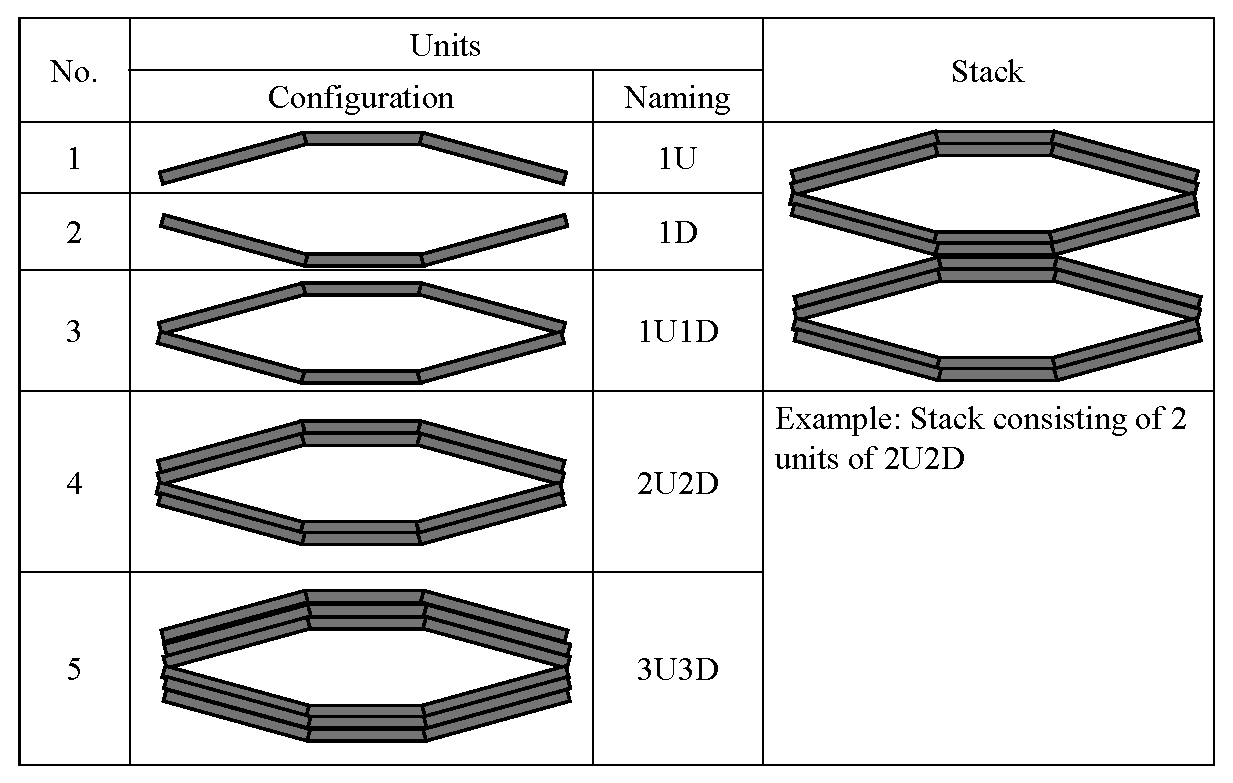
\includegraphics[scale=0.5]{WasherNomenclature.eps}
    \caption{Nomenclature used for Belleville washer units and stacks}
    \label{fig:WasherNomenclature}
\end{figure}

Then washers are nested with the cones oriented in the same direction, as for example in the top or bottom half of a 2U2D unit, they act in \textit{parallel} since when a load is applied, their deformations are the same. When the cone orientations are opposite, as for example with the two washers in a 1U1D unit, they are in series, since they see the same force and their deformations are additive. Thus, a stack can be viewed as a series-parallel arrangement of washers. If the washers were ideal springs, the stiffness of a stack can be calculated using series-parallel combinations of the stiffnesses of the constituent springs (as will be seen in section \ref{sec:washerstackforcedisp}), washers, particularly when nested are not linear springs and exhibit hysteresis, so such a calculation of stiffness would only be approximate). The strength (flattening load) of a stack is determined by the weakest parallel combination in the stack.

\begin{figure}[t]
    \centering
    \includegraphics[scale=0.8]{CVTDrawing.eps}
    \caption{Capacitive voltage transformer (CVT) provided by Seattle City Light and used in shake table experiments described in section \ref{sec:shaketableexperiments}.}
    \label{fig:CVTDrawing}
\end{figure}

\subsection{Analysis and design questions}\label{subsec:analysisdesignquestions}
The findings reported here must ultimately guide the selection of washer stacks the provide the desired level of seismic protection. This is the design question, given (a) an equipment, (b) its support structure, (c) seismic input (design spectrum) and (d) performance specifications (max base moment, max terminal displacement etc.), design a Belleville washer stack so that the system response meets the specifications.\\

A prerequisite to approaching this design question is being able to answer the analysis question, given (a) an equipment, (b), its support structure, (c) seismic input (ground motion record) and (d) a specific Belleville washer configuration, compute the response of this system (accelerations, base moments, terminal displacements etc.). Hence the emphasis of this project is more on this analysis question and support for the analysis process from physical experimental measurements, with a focus as noted above on “rigid” structures, in particular a CVT.

\subsection{Organization of the report}\label{subsec:reportorganization}
This report is organized as follows. As noted above, the main goal of this project is to develop an analysis-based systematic approach for design of a Belleville washer seismic protective system. The report is therefore structured around an analysis procedure. This procedure is summarized upfront in section \ref{sec:analysisprocedure}, and the various steps in this procedure are expounded in subsequent chapters. Characterizing the force-displacement hysteresis of a single stack of washers through cyclic loading tests is presented in section \ref{sec:washerstackforcedisp}. Shake table experiments to characterized dynamic seismic response of a CVT equipment with Belleville washer stacks, including setup, instrumentation and specific steps for installing the washer stacks, are described in section \ref{sec:shaketableexperiments}. In section \ref{sec:nonlinmodelanalysis}, a nonlinear dynamic model of the CVT with Belleville washer stacks is developed, and predictions from the model are compared with measurements from shake table experiments. An important note is that all the information needed for this model can be obtained from the washer characterization data from section \ref{sec:washerstackforcedisp}, the type of information that can be readily obtained. In section \ref{sec:equilinmodel}, a linearized model based on equivalent stiffness and damping is developed that may be more conducive for practical use than the nonlinear model in section \ref{sec:nonlinmodelanalysis}; this linear model can also be developed simply for the characterization data in section \ref{sec:washerstackforcedisp}. The approach taken in this report to analyze substation equipment with Belleville washer seismic protective systems loosely parallels that in ASCE 7 for seismically isolated structures; this is pointed out in section \ref{sec:equilinmodel} to lend credence to the proposed approach relative to well-established procedures in seismic standards. Finally in section \ref{sec:conclusion}, a summary is provided, and some outstanding questions are identified.

\section{Proposed analysis procedure}\label{sec:analysisprocedure}
The main goal of this project is to develop an analysis-based systematic approach for design of a Belleville washer seismic protective system. Therefore, in this chapter, a proposed analysis procedure is laid out. This serves to tie together the different steps and experimental support for these steps discussed in subsequent chapters. The following is the proposed analysis procedure:\\

\noindent Given (a) an equipment, (b) its support structure, (c) seismic input (ground motion record), (d) 
Belleville washer configuration
\begin{enumerate}
  \item Determine the force-displacement response of the stack.
  \begin{itemize}
    \item In this project, we have done this by testing the stack in a material test machine (see section \ref{sec:washerstackforcedisp}).
    \item This is a hysteretic behavior.
  \end{itemize}
  \item Compute the moment-rotation behavior of the assembly of washer stacks (see section \ref{sec:nonlinmodelanalysis}).
      \begin{itemize}
        \item This can be done, for example, in an Excel spreadsheet.
        \item In this project, special instrumentation has been used to experimentally verify the relationship between the stack force-displacement behavior and the system moment-rotation behavior (see section \ref{sec:shaketableexperiments}).
      \end{itemize}
  \item Model this moment-rotation behavior – two possible approaches.
      \begin{itemize}
        \item Fit a hysteresis model (section \ref{sec:nonlinmodelanalysis}).
        \item Compute an “equivalent” stiffness and damping (section \ref{sec:equilinmodel}).
        \item Both approaches have been verified in this project; it has also been verified that this equivalent stiffness and damping agrees well with fitting a linear model to the 
measured response.
      \end{itemize}
  \item Compute the system response – three approaches are possible.
  \begin{itemize}
    \item  Nonlinear time-history analysis with the hysteresis model for the washer arrangement (section \ref{sec:nonlinmodelanalysis}).
    \item Linear time history analysis with the equivalent stiffness and damping.
    \item Response spectrum analysis with the equivalent stiffness and damping ((section \ref{sec:equilinmodel}). This together with the equivalent stiffness and damping resemble ASCE 7 process for base isolation (Chapter -)
    \item In the project, it has been verified that the three approaches produce close responses.
  \end{itemize}
\end{enumerate}

\section{Cyclic force-displacement behavior of washer stacks}\label{sec:washerstackforcedisp}
This chapter is on the measurement of force-displacement behavior of Belleville washer stacks. As will be seen in sections \ref{sec:nonlinmodelanalysis} and \ref{sec:equilinmodel}, this is the primary information required to predict the seismic response of rigid equipment (besides mass, moment of inertia of the equipment itself and support structure stiffness).\\

The force displacement response of a washer stack is obtained here by applying cyclic compressive loading to the stack in a materials testing machine. At first, this was done by simply compressing the stack between loading plates as shown in Figure 3-1(a). The resulting force-displacement curves of Figure 3-1(b) showed changes in slope that weren’t observed in force-displacement measurements of the same stack in shake table tests (the special instrument designed to measure this response in situ under the equipment in the shake table test is discussed in section \ref{sec:shaketableexperiments}). This is likely because of slight misalignment between washers in the stack initially that corrects itself during the loading. To avoid this, an alternative approach was devised, where the compressive loading was applied to the stack through a loading frame and guiding rod as illustrated in Figure 3-2(a). This arrangement is closer to how the washer stack is installed under the equipment. The guiding rod prevents any initial misalignment and subsequent realignment. The resulting force-displacement measurement, shown in Figure 3-2(b), does not have any unexpected changes in slope. Indeed the in situ measurements from the shake table tests follow these curves closely as seen in Figure 3-3.\\
%%%%%%%%%% Figure 3-1
%%%%%%%%%% Figure 3-2
%%%%%%%%%% Figure 3-3
%%%%%%%%%% Figure 3-4
Figure 3-4 shows force-displacement curves for two configurations of the K1750-J-057 washers. They exhibit the reduction in stiffness with loading noted in Figure \ref{fig:Forcedisponewasher} due to their higher $h$/$t$ ratio.

\section{Shake table experiments}\label{sec:shaketableexperiments}
In this chapter, shake table experiments on the CVT equipped with Belleville washer stacks are described. The experimental setup, instrumentation, and washer installation process are detailed. The primary purpose of these experiments is to obtain measurements in support of the analysis procedure outlined in section \ref{sec:analysisprocedure}. Consequently, special instruments were used to measure the washer response in situ. Instrumentation was also designed with redundancy in mind, so that the same quantity is measured by multiple means and can be cross-checked. Some other checks such as sums of forces are moments are perform to confirm the integrity of the measurements.
\subsection{Test setup}
Figure \ref{fig:Shaketablesetup} shows the CVT mounted on the shake table. The CVT is mounted on a pedestal referred to as the “spool”, which in turn is mounted on the shake table. The spool consists of a 10-in diameter ½-in thick 16.5-in tall steel tube with a 22in×17in steel plate welded on top (to match the base dimensions of the CVT). Figure \ref{fig:Shaketablesetup} also shows the direction convention $X$ along the East-West direction, Y along the North-South direction and $Z$ along the vertical direction. The distance between the mounting holes at the base of the CVT is greater in the $Y$ direction than in $X$ direction (resulting, for example, in the $Y$ frequency direction than in the $X$ direction). The Belleville washer stacks are installed between the CVT base and the spool, details of which are elaborated below.
\begin{figure}[t]
    \centering
    \includegraphics[scale=0.6]{Shaketablesetup.eps}
    \caption{CVT mounted on shake table}
    \label{fig:Shaketablesetup}
\end{figure}
\subsection{Instrumentation}
An overview of response quantities measured and corresponding instrumentation is provided in Figure \ref{fig:Instrumentation}. Table \ref{tab:instrumentation} contains a detailed summary. In addition to these response quantities that are measured directly, further response quantities are derived indirectly from them. These quantities as well as the process used to derive them are summarized in Table \ref{tab:deriveresponsequant}. A specialized instrument in Table \ref{tab:instrumentation}, designed in this project to measure the force in a washer stack in situ is the Load Washer Alternate (LWA) shown in Figure \ref{fig:LWA}. It consists of a frame made of a frame consisting of two plates and two ¾-in threaded rods. The guiding rod of the Belleville washer stacks goes through a hole in the top plate, and connects to a load cell attached to the bottom plate. When the washer stack right above the top plate is compressed, the guiding rod develops tension that is measured by the load cell. Thus the load cell measures the compression in the Belleville washer stack below the spool plate. 

\begin{figure}
\centering
\hfil
\subfloat[Summary of instruments]{\includegraphics[scale=0.65]{Instruments.eps}%
\label{fig:Instruments}}
\hfil
\subfloat[Closeup of yellow box in (a)]{\raisebox{5em}{\includegraphics[scale=0.6]{InstrumentsCloseup.eps}%
\label{fig:InstrumentsCloseup}}}
\caption{Instrumentation details}
\label{fig:Instrumentation}
\end{figure}

\begin{table}[ht]
\caption{\label{tab:instrumentation} Summary of measured response quantities and corresponding instruments}
\begin{center}   
\begin{tabular}{cm{6cm}m{9cm}} 
 \toprule
No. & Response quantity & Instrument\\ \midrule
1 & Top $X$ and $Y$ displacement components & String potentiometers attached to frames outside the shake table, so these measure 
absolute displacements \\ \midrule
2 & Top $X$ and $Y$ acceleration components & One 3D accelerometer\\\midrule
3 & $X$ and $Y$ accelerations at insulator mid-height & Two 1D accelerometers\\\midrule
4 & $Z$ accelerations at N, S, E, W locations on CVT box & Four 1D accelerometers\\\midrule
5 & Insulator base moment & Strain gages at N, S, E, W locations at insulator base, calibrated to measure base moment\\\midrule
6 & Displacements at 4 locations of the base of the CVT relative to the spool plate & Four linear potentiometers\\\midrule
7 & Tension forces in rods going through the four washer stacks & Four specially designed instruments called “load washer alternates” LWAs (see below)\\\midrule
8 & Two bending moment components in the spool ($\Mspool$) & Two full-bridge strain gage circuits, one for $X$ bending moment and the other for $Y$ \\\midrule
9 & Shake table accelerations & 3D accelerometers\\\midrule
10 & Shake table displacement & String potentiometers\\
\bottomrule
\end{tabular}
\end{center}
\end{table}

\begin{table}[ht]
\caption{\label{tab:deriveresponsequant} Response quantities derived indirectly from measurements}
\begin{center}   
\begin{tabular}{cm{6cm}cm{7cm}} 
 \toprule
No. & Derived response quantity & Symbol* & Method of computation\\ \midrule
i & Rigid-body translational and rotational acceleration of CVT at center of mass & $\xtddot$, $\ddot{\theta}$ & Linear fit to acceleration components rows 2--4 
in Table \ref{tab:instrumentation}. A good fit here demonstrates the 
CVT can be idealized as a rigid body. \\ \midrule
ii & Total rotation of CVT & $\theta$ & Linear fit to CVT displacements (row 1) and shake table displacements (row 10) in Table \ref{tab:instrumentation}. \\ \midrule
iii & Rotation of CVT relative to spool plate & $\thetaw$ & Linear fit to displacements in row 6 of Table \ref{tab:instrumentation}. \\ \midrule
iv & Restoring moment generated by washer stacks (and spool plate) & $\MCVT$ & Twice the moment computed from the four 
LWAs (row 7 of Table \ref{tab:instrumentation}, see Figure 4-3 for 
details). \\ \midrule
v &  Deflection of spool plate &  & Difference of rows ii and iii above \\
\bottomrule
\multicolumn{4}{l}{\small{\makecell[l]{*The symbols listed here are in reference to dynamics in the $X$ (East-West) direction, corresponding quantities in the \\ $Y$ (North-South) direction will be labeled similarly, but not shown here}}}
\end{tabular}
\end{center}
\end{table}

\begin{figure}
    \centering
    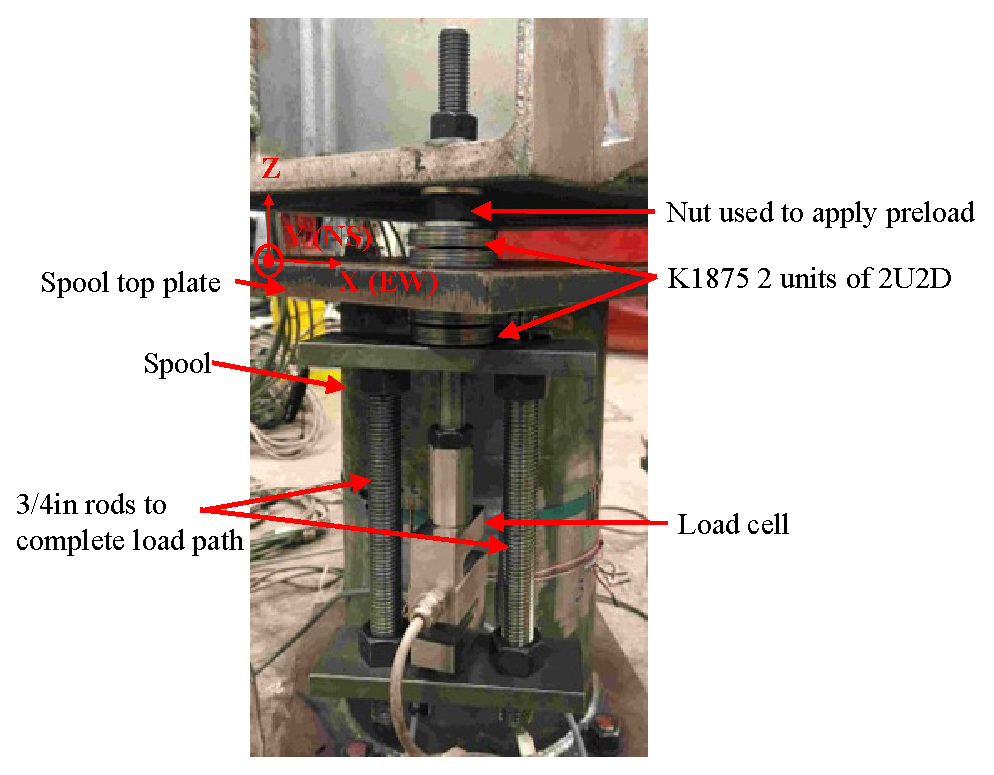
\includegraphics[scale=0.62]{LWA.eps}
    \caption{Details of Load Washer Alternate (LWA) and preloading process}
    \label{fig:LWA}
\end{figure}
\subsection{Determination of CVT inertia properties}
For further analysis, the mass, mass moment of inertia and center of mass position of the CVT must be determined. The mass is obtained simply from the measured weight. The center of mass position is determined by balancing the CVT horizontally using a crane. The mass moment of inertia is computed from the frequency measured by mounting the CVT on springs of known stiffness (Figure \ref{fig:CVTonspring}) using the method outlined in Figure 4-5. A summary of the inertia properties of the CVT is shown in Table \ref{tab:CVTinertia}.
\begin{figure}
    \centering
    \includegraphics[scale=0.62]{CVTonspring.eps}
    \caption{CVT mounted on springs to estimate mass moment of inertia indirectly from measured frequency}
    \label{fig:CVTonspring}
\end{figure}

\begin{table}[ht]
\caption{\label{tab:CVTinertia} Summary of CVT inertia properties}
\begin{center}   
\begin{tabular}{cm{7.5cm}c} 
 \toprule
Parameter (Unit) & Description & Value\\ \midrule
$m$ (lb-s$^2$/in) & Mass & 940/386.4 \\ \midrule
$\hCG$ (in) & Height of center of mass from CVT base & 35-1/16 \\ \midrule
$I$ (lb-s$^2$-in) & Mass moment of inertia about center of rotation & 5500 \\ \midrule
$\Izero$ (lb-s$^2$-in) & Mass moment of inertia about center of mass & 2500 \\
\bottomrule
\end{tabular}
\end{center}
\end{table}
\subsection{Washer stack installation}
Special care is exercised in controlling the preload when installing the Belleville washer stacks. The stacks are installed on the spool plate with out the CVT present. The stacks at each corner are preloaded independently by tightening the nut at the top (Figure \ref{fig:LWA}) by a prescribed number of turns corresponding to fraction of flattening displacement targeted in the washer stacks. The 
force in the bottom stack is simultaneously monitored using the LWA to make sure that the load corresponds to the stack deflections in accordance with the force-deformation relationship measured in the tests described in section \ref{sec:washerstackforcedisp}. The CVT is then seated on the four top nuts, and fixed in place using four nuts above the CVT base plate.

\subsection{Test configurations and protocol}
Pull tests were performed in the X and Y directions with the CVT fixed directly to the spool plate to calibrate to the bending moment load cells in the spool and the strain gages at the insulator base to bending moment. The washer configurations shown in Table \ref{tab:washerconfigsummary} were tested. All configurations were double acting – there were washer stacks above and below the spool plate.
\begin{table}[ht]
\caption{\label{tab:washerconfigsummary}Summary of configurations tested}
\begin{center}   
\begin{tabular}{ccc} 
 \toprule
Washer & Configuration & Pre-load (\% of flattening load)\\ \midrule
\multirow{3}{*}{K1875-G-086} & \multirow{3}{*}{2 units of 2U2D} & 0lb (0\%) \\
& & 500lb (25\%) \\
& & 1000lb (50\%) \\ \midrule
\multirow{2}{*}{K1750-J-057} & \multirow{3}{*}{3 units of 3U3D} & 500lb (17\%) \\
& & 1500lb (50\%) \\
\bottomrule
%\multicolumn{3}{l}{\small{$^1$Obtained from \cite{kote2019model}}}
\end{tabular}
\end{center}
\end{table}
For each configuration, a sequence of tests consisting of low-level broad-band random input (for baseline system identification) and the CERL ground motion with increasing amplitude levels (culminating at 0.5g) were applied first in the X direction and then in the Y direction. The 5\%-damped test response spectra of the applied motion are shown in Figure 4-6.

\section{Nonlinear modeling and analysis}\label{sec:nonlinmodelanalysis}

\section{Equivalent linear modeling}\label{sec:equilinmodel}

\section{Summary and concluding remarks}\label{sec:conclusion}

\subsection{Executive summary}\label{subsec:execsummary}
A modeling procedure has been developed to predict the seismic response of rigid equipment such as CVTs equipped with Belleville washer stacks at the base for seismic protection. The procedure allows for nonlinear dynamic analysis or an equivalent linear analysis, and is outlined in section \ref{sec:analysisprocedure}. The starting points are (a) the force-displacement hysteretic behavior of an individual stack that can be readily obtained by cyclic loading in a materials test machine, (b) inertia properties of the CVT – mass, mass moment of inertial and center of mass location. With this, the seismic response can be predicted reliably. This has been validated with experiments on an earthquake simulator (shake table). Special instrumentation was developed to obtained detailed in situ measurements of the behavior of the washer stacks in the shake table experiments. Validation using these measurements provides confidence that the analysis procedure can be used to inform decisions when installing Belleville washer devices in the field. The process also parallels procedures in ASCE 7-16 for seismic isolators.\\

The washer stacks essentially act as seismic isolators, reducing the frequency and increasing the damping. They are effective in reducing the insulator base moment. As is the case with seismic isolation systems, reduction is base moment has to be traded off with increase in terminal displacement.

\subsection{Outstanding research questions}\label{subsec:outstandingquestions}
Some outstanding research questions remain:\\

Testing and modeling with different washer types; only one washer type has been studied completely (K1875-G-086). A second washer type has been studied partially (K1750-J-057), but some issues were discovered and are being remedied. It will be useful to complete the study with 
the K1750 washer type, as well as one other washer type from a different vendor. \\

Testing and modeling beyond flattening load: When subject to earthquake larger than what the spring washer protective system is designed for, the washer is likely to flatten, causing a different type of dynamics. It will be useful to study this performance under extreme loading. This is similar to when a base isolation system hits its displacement limit, which is considered it the design.\\

Testing and modeling single acting configuration: Thus far, we have only test cases with the spring washers in a single acting configuration, but that one configuration revealed promising 
behavior consisting of flag-shaped hysteretic behavior. It will be useful to study this further.
%\bibliographystyle{IEEEtran}
\bibliography{References}
	
\end{document} 